\section{Metodología}

\textbf{Metodología en V}\\
Para el desarrollo del sistema se tomará en cuenta la metodología en V para el desarrollo de software, partiendo de la definición de requerimientos funcionales y no funcionales, trazando un plan para el modelado del sistema mediante casos de uso, comprendiendo las limitaciones, identificando el impacto del mismo y previendo posibles cambios. Se hace un diseño del sistema con la ayuda de toda la información recogida sobre requisitos y análisis, donde veremos el sistema de manera modular, teniendo la ventaja de identificar los errores en una sección específica de este. Posteriormente el diseño es implementado con el lenguaje de programación elegido, obteniendo programas ejecutables capaces de ofrecer la funcionalidad esperada. A su vez cada etapa va a ser sometida a pruebas unitarias, integradoras y finalmente, del sistema para validar el análisis y diseño previamente hecho de manera ascendente \citep{Metodologia1}.

Las pruebas de cada nivel son descritas a continuación:

Donde:
\begin{itemize}

    \item Pruebas unitarias/modulares: estas pruebas comprueban que todas las funcionalidades especificadas en el diseño del componente sean correctas y cubiertas, estas pruebas son realizadas por el desarrollador del componente.
    
    \item Pruebas de integración/interfaz:
    Conforme los módulos son implementados y probados de manera unitaria, se procede a probar su funcionalidad de manera conjunta, estas pruebas están enfocadas a:
    
    \begin{itemize}
        \item Que espera un componente de otro componente, en termino de servicios.
        \item Como es que estos servicios serán solicitados.
        \item Como es que estos servicios serán entregados.
        \item El manejo de errores por condiciones inesperadas.
    \end{itemize}
    
    Las pruebas deben corroborar el correcto funcionamiento de todas las interfaces entre componentes, al tener todos los componentes y sus interfaces terminadas tendremos como resultado el sistema completo, estas pruebas pueden ser realizadas por el desarrollador del componente.
    
    \item Pruebas del sistema: Una vez el sistema ha sido construido, debe ser probado contra las especificaciones del sistema para comprobar que cubra las funcionalidades requeridas.\\
    Esta parte se enfoca en probar el sistema de manera monolítica y debe incluir las pruebas para validar los requerimientos no funcionales.

    \item Pruebas de validación: similar a las pruebas del sistema, pero hay un cambio en el enfoque, ya que estas comprueban que el sistema cumple con lo requerido, estas pruebas son realizadas por el usuario final del sistema.

\end{itemize}

\\
\begin{figure}[H]
	\centering
	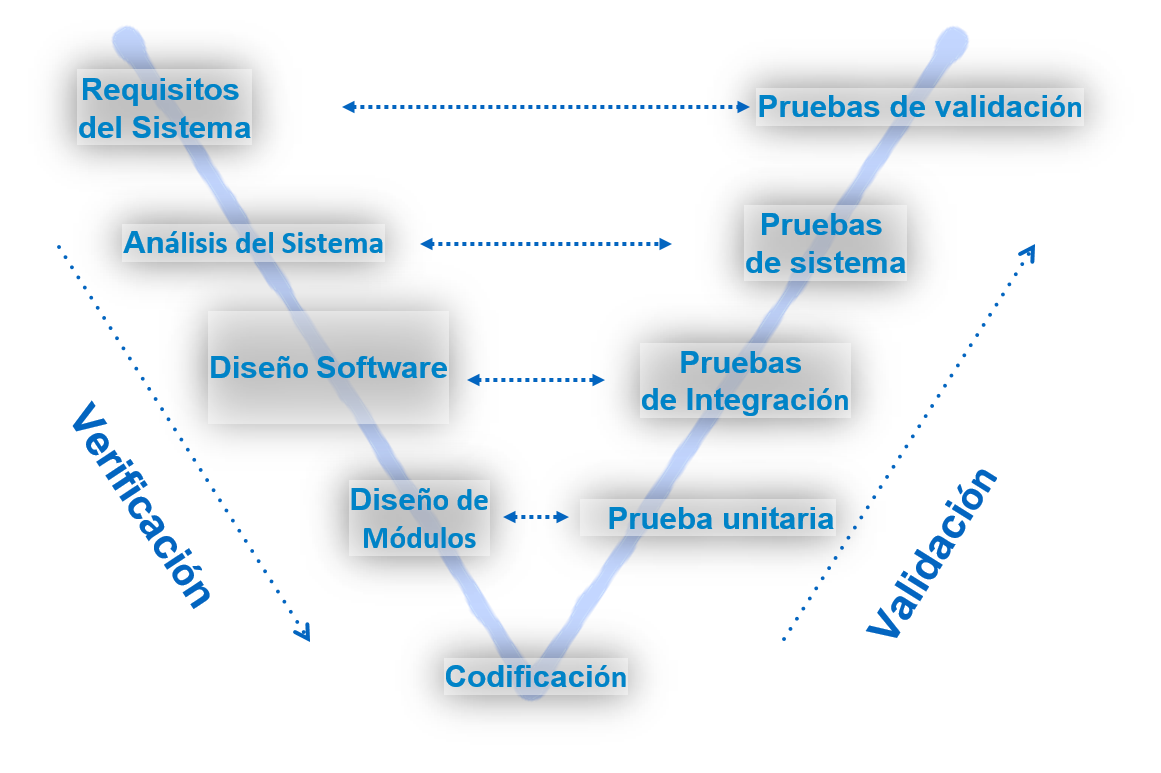
\includegraphics[scale=.5]{Capitulo3/img/vmodel.png}
	\caption{Metodología en V}
	\label{fig:ModeloIncremental}
\end{figure}


Este tipo de modelo se utilizará debido a que los incrementos nos permiten desarrollar el sistema desde su parte mas fundamental hasta tener el sistema completo y funcionando, obteniendo un entregable en cada uno de los incrementos.
\\
Los incrementos que se realizarán serán los siguientes:
\\
\begin{enumerate}
	\item Se realizará el módulo del sensor el cual consiste en el análisis del sensor de flujo, del microcontrolador a utilizar y la forma de comunicación con la aplicación móvil para el envío del dato de la medición obtenida.
	\item Se hará el diseño y programación para realizar la comunicación entre el sensor y la aplicación y se realizarán las pruebas unitarias pertinentes para asegurar que la medición y comunicación sean correctos.
	\item Se realizará módulo de la aplicación móvil el cual consiste en el análisis y diseño de la aplicación móvil para la obtención de datos, se realizará la programación de la interfaz de la aplicación móvil con la cual el usuario podrá visualizar los datos y se realizaran las pruebas pertinentes.
	\item Se continuará con el análisis, diseño y programación del submódulo de usuarios, en el cual se tendrá una aplicación móvil en la cual el usuario pueda interactuar de una forma fácil y eficiente con el sistema.
	\item Se realizará el análisis, diseño y programación del submódulo para la geolocalización de los establecimientos.
	\item Se realizara el análisis y diseño para el envío y recepción de datos entre la aplicación móvil y el servidor web y se realizarán las pruebas de integración de todo el módulo de la aplicación móvil.
	\item Se realizará el módulo servidor web el cual consiste en el análisis, diseños y programación de la recepción de los datos obtenidos, asimismo se realizarán las pruebas unitarias del incremento en cuestión.
	\item Se continuará con el módulo servidor web con el análisis, diseño y programación para la clasificación de los establecimientos según los resultados obtenidos y se realizarán tanto pruebas unitarias del módulo servidor web..
	\item En este incremento se harán las pruebas de integración del sistema.	
\end{enumerate}
